\documentclass[12pt,halfline,a4paper]{ouparticle}
\begin{document}
%equation number = section.section.number
\numberwithin{equation}{section}
%spacing between paragraph
\setlength{\parskip}{0.5em}
\title{Renormalization of $n$-point correlation function}
%define the theroem environment
\newtheorem{theorem}{Theorem}
\newtheorem{definition}{Definition}
%define the lemma environment	
\newtheorem{lemma}{Lemma}
\author{%
\name{Yeonjoon Kim}
\name{Haemin Jeong}
}


\date{\today}

\maketitle


\section{Introduction}
\label{sec1}
The most difficult part of understanding renormalization is that it lacks an intuitive explanation. 
There are many misunderstandings and lumps in the concepts of renormalization,
for example, treat renormalization as a mathematical trick to make the theory finite, which also can be makes that motivate us to be enroll to this class.

As we learned in class, Kenneth Wilson's work is shine the lights on intuitive perspective on this renormalization process.
Which means ``Different Equivalent physics on Different Scale".
wilsonian renormalization is often it described by flow on parameter space of lagrangian by variation in the energy scale. 
Which we called the ``Renormalization Group flow".
Now that we have an intuitive view, let's take it one step further.	
Of course some Lagrangian gives us the distinct physics by path integral, but in what sense?

Think about all the experiments we've done, we've called them `colliders'. LEP, the $e^+e^-$ collider, even the case of HERA ($e^- p$ collider), we think of them as collisions of point-like particles, although the proton is actually a non-perturbative soup.
I think, at least in a somewhat classical sense, this should be in the picture of particle interaction for sake of intuition.


Basic building of this is the $n$-point correlation function, which is directly related to scattering amplitude by LSZ reduction formula. let we have the scalar field theory.
the LSZ reduction formula is given by
\begin{align}\begin{split}
\label{LSZ}
\langle f| i\rangle = i^{n+n^\prime}\int e^{ik_1x_1}(-\partial^2_1+m^2)&...\times\\e^{-ik^\prime_1x^\prime_1}(-\partial^2_{1^\prime}+m^2)...\langle 0|&T\phi(x_1)...\phi(x_n)\phi(x^\prime_1)...\phi(x^\prime_{n^\prime})|0\rangle
\end{split}\end{align}
where $|i\rangle$ and $|f\rangle$ are the initial and final states, respectively, defined by $n^\prime$ and $n$ number of incoming and outgoing particles. Thus LSZ reduction formula is the bridge between the scattering amplitude and the $n+n^\prime$-point correlation function.

while $n-$point correlation function is defined by path integral. from now, we will work in the euclidean spacetime as usual.
\begin{align}\begin{split}
\label{correlation}
\langle 0|T\phi(x_1)...\phi(x_n)|0\rangle = \frac{1}{Z[\mathbf{j}]}\frac{\delta^{2n}}{\delta(x_1)...\delta(x_n)}\int [\mathcal{D}\phi] e^{-S_E[\phi]+\mathbf{j}\cdot\phi}\bigg\rvert_{\mathbf{j}=0}
\end{split}\end{align}
So the new question is, how does the $n$-point correlation function change when we change the energy scale? In other words, how does it change under Wilsonian RG?
This may help the more intuitive picture of corse-graining as $n$-point correlation that function directly related to scattering amplitude, particle experiments.

\section{Renormalization Group Flow}
\label{sec2}

What he actually do in his paper?
First, Develop the flow equation of the lagrangian through the parameter space in changes of corresponding energy scale.
Second, show the coeffcients of effective lagrangian at enregy scale $\mu$ has $\Lambda\rightarrow \infty$ limit, i.e. renormalizable, and also for the $n$-point correlation function.
Despite his 1984 paper devote most space for the second part, but we think more important part is the former. 
Hence we won't follow the every steps of his proof to second part in detail, rather stress the first part, intuitive understanding of his flow equation.
But for now, let's start with the basic concept of RG flow to see the everythings in the same way as the Polchinski's.

RG Flow is the actually the ``flow" of lagrangian, like a particle flow through the streamline with the some variable $t$.
But in the case of RG flow, our lagrangian flow along the parameter space through the curve that represents the equivalent physics,
as the function of energy cutoff variable $\mu$.

Now Let's rephrase the term ``Renormalizability" in this picture. lagrangian $\mathcal L$ can include the infinitely many number of terms, hence the dimension of the parameter space is also infinite.
But non-renormalizable term, says, ``irrelevant'' term, suppressed by the inverse power of bare cutoff $\Lambda$.
Therefore infinite-dimensional mainfold tends to shrinks to the finite-dimensional manifold that which has the dimension of number of relevent and marginal terms.
Hence whether the theory is started from the point of the parameter space, it will attracted to renormalizable manifold at the IR side. What Polchinski shows is that for our effective lagrangian $\mathcal{L}_\mu$ in renormalizable manifold in IR side,
and also there is a starting point for a given $\Lambda_0$ that flow starts, in rigourous manner, and also for the $n$-point correlation function.

Let's start with Polchinski's toy argument. For our regular $d=4$ spacetime with scalar theory with 4 and 6-point interaction, says
\begin{equation}
	\mathcal{L}_{\text{int}}=g_4\phi^4+g_6\phi^6
\end{equation}
Which is marginal and irrelevant term, respectively.
First we are going to behaviour of flow on 2D parameter space, and will generalize this in later chapter.
We can deduce the scailing dependence of the coupling constant $g_4$ and $g_6$ by the dimensional analysis.
Since $\phi$ has the mass dimension of $1$, $g_4$ and $g_6$ has the mass dimension of $0$ and $-2$, respectively.
Therfore we can write
\begin{align}\begin{split}
	&\frac{d g_4}{d \ln \Lambda} = \beta_4(g_4,\Lambda^2g_6)\\
	&\frac{d g_6}{d \ln \Lambda} = \Lambda^{-2}\beta_6(g_4,\Lambda^2g_6)
\end{split}\end{align}
This can be inferred by the simple dimensional analysis. Define the dimensionless constant, $\lambda_4=g_4$ and $\lambda_6=\Lambda^{2}g_6$. Then above equation can be written as
\begin{align}\begin{split}
	\label{eq:damping}
	&\frac{d \lambda_4}{d \ln \Lambda} = \beta_4(\lambda_4,\lambda_6)\\
	&\frac{d \lambda_6}{d \ln \Lambda} -2\lambda_6 = \beta_6(\lambda_4,\lambda_6)
\end{split}\end{align}
We can already see that hint of the irrelevant behaviour of $\lambda_6$ here. Consider $\beta_6$ is very small. Than $-2\times$ part contributes like a damping force to the evolution of $\lambda_6$, like
\begin{equation}
	\frac{d\lambda_6}{\lambda_6}=2d\ln\Lambda
\end{equation}
means that $\lambda_6$ will be suppressed by the inverse power of $\Lambda^2$, $\lambda_6(\Lambda)\sim\Lambda^{-2}\lambda_6(\mu)$.

now consider the two trajectories, $\lambda^\prime$ and $\lambda^{\prime\prime}$. We can expand the $\beta_i$ using the taylor expansion, at some point $\lambda^*$.
Then we can write the evolution of small amount, $\epsilon$, which the difference of the two trajectories, $\epsilon_i=-\lambda_i^\prime+\lambda_i^{\prime\prime}$.
\begin{align}\begin{split}
\frac{d \epsilon_4}{d\ln\Lambda}&=\frac{\partial\beta_4}{\partial\lambda_4}\bigg\lvert_{\lambda^\prime}\epsilon_4+\frac{\partial\beta_4}{\partial\lambda_6}\bigg\lvert_{\lambda^\prime}\epsilon_6\\
\frac{d \epsilon_6}{d\ln\Lambda}&=\frac{\partial\beta_4}{\partial\lambda_4}\bigg\lvert_{\lambda^\prime}\epsilon_4+\bigg(\frac{\partial\beta_4}{\partial\lambda_6}\bigg\lvert_{\lambda^\prime}+2\bigg)\epsilon_6
\end{split}\end{align}
This is no more than linear approximation of the difference of the two trajectories and their evolutions.
What we have to answer is: these two trajectories \textbf{attracts} each others? 
More precisely, does these trajectories shrinks down to the 1-dimesional manifold, i.e. $g_6$ is irrelevant while $g_4$ is relevant?
The answer might seems yes, because same logic as the equation \ref{eq:damping}, factor of $2$ in the second equation acts like a damping force agian.
but this is not sufficient to just show $\epsilon_6$ goes zero at some energy scale $\Lambda$, because relevant part of $\epsilon_4$ can evolves quite differentely, 
%for example is there are IR fixed point at origin and flow is radialy inward(like a electric field near the point charge), $\epsilon_6$ will go 0 at some energy scale but the parameter space is not clearly 1-dimensional even in IR region, 
%this is not we usually consider in language of renormalizability.

Instead, consider one more variable $\xi_i$, which is changes due to relevant part is eliminated from the $\epsilon$. This procedure is can be understood in analogy with Gram-Schmidt orthogonalization.
in 2 dimension, orthognal part of vector $\mathbf{a}$ respect to $\mathbf{b}$ can be extracted by $\mathbf{a}-(\mathbf{a}\cdot\mathbf{b})/(\mathbf{b}\cdot\mathbf{b})\mathbf{b}$, 
therefore our new variable will calculated by $\xi=\epsilon_i-\#d\lambda^\prime_i/d\Lambda$, with appropriate numerical factor $\#$.
to make $\epsilon_4=0$, $\#$ is clearly $\epsilon_4/(d\lambda^\prime_4/d\Lambda)$. Then $\xi_6$ will be

\begin{equation}
	\label{xi6}
	\xi_6=\epsilon_6-\frac{d\lambda^\prime_6}{d\Lambda}\frac{\epsilon_4}{d\lambda^\prime_4/d\Lambda}
\end{equation}
\begin{figure}
	\centering
	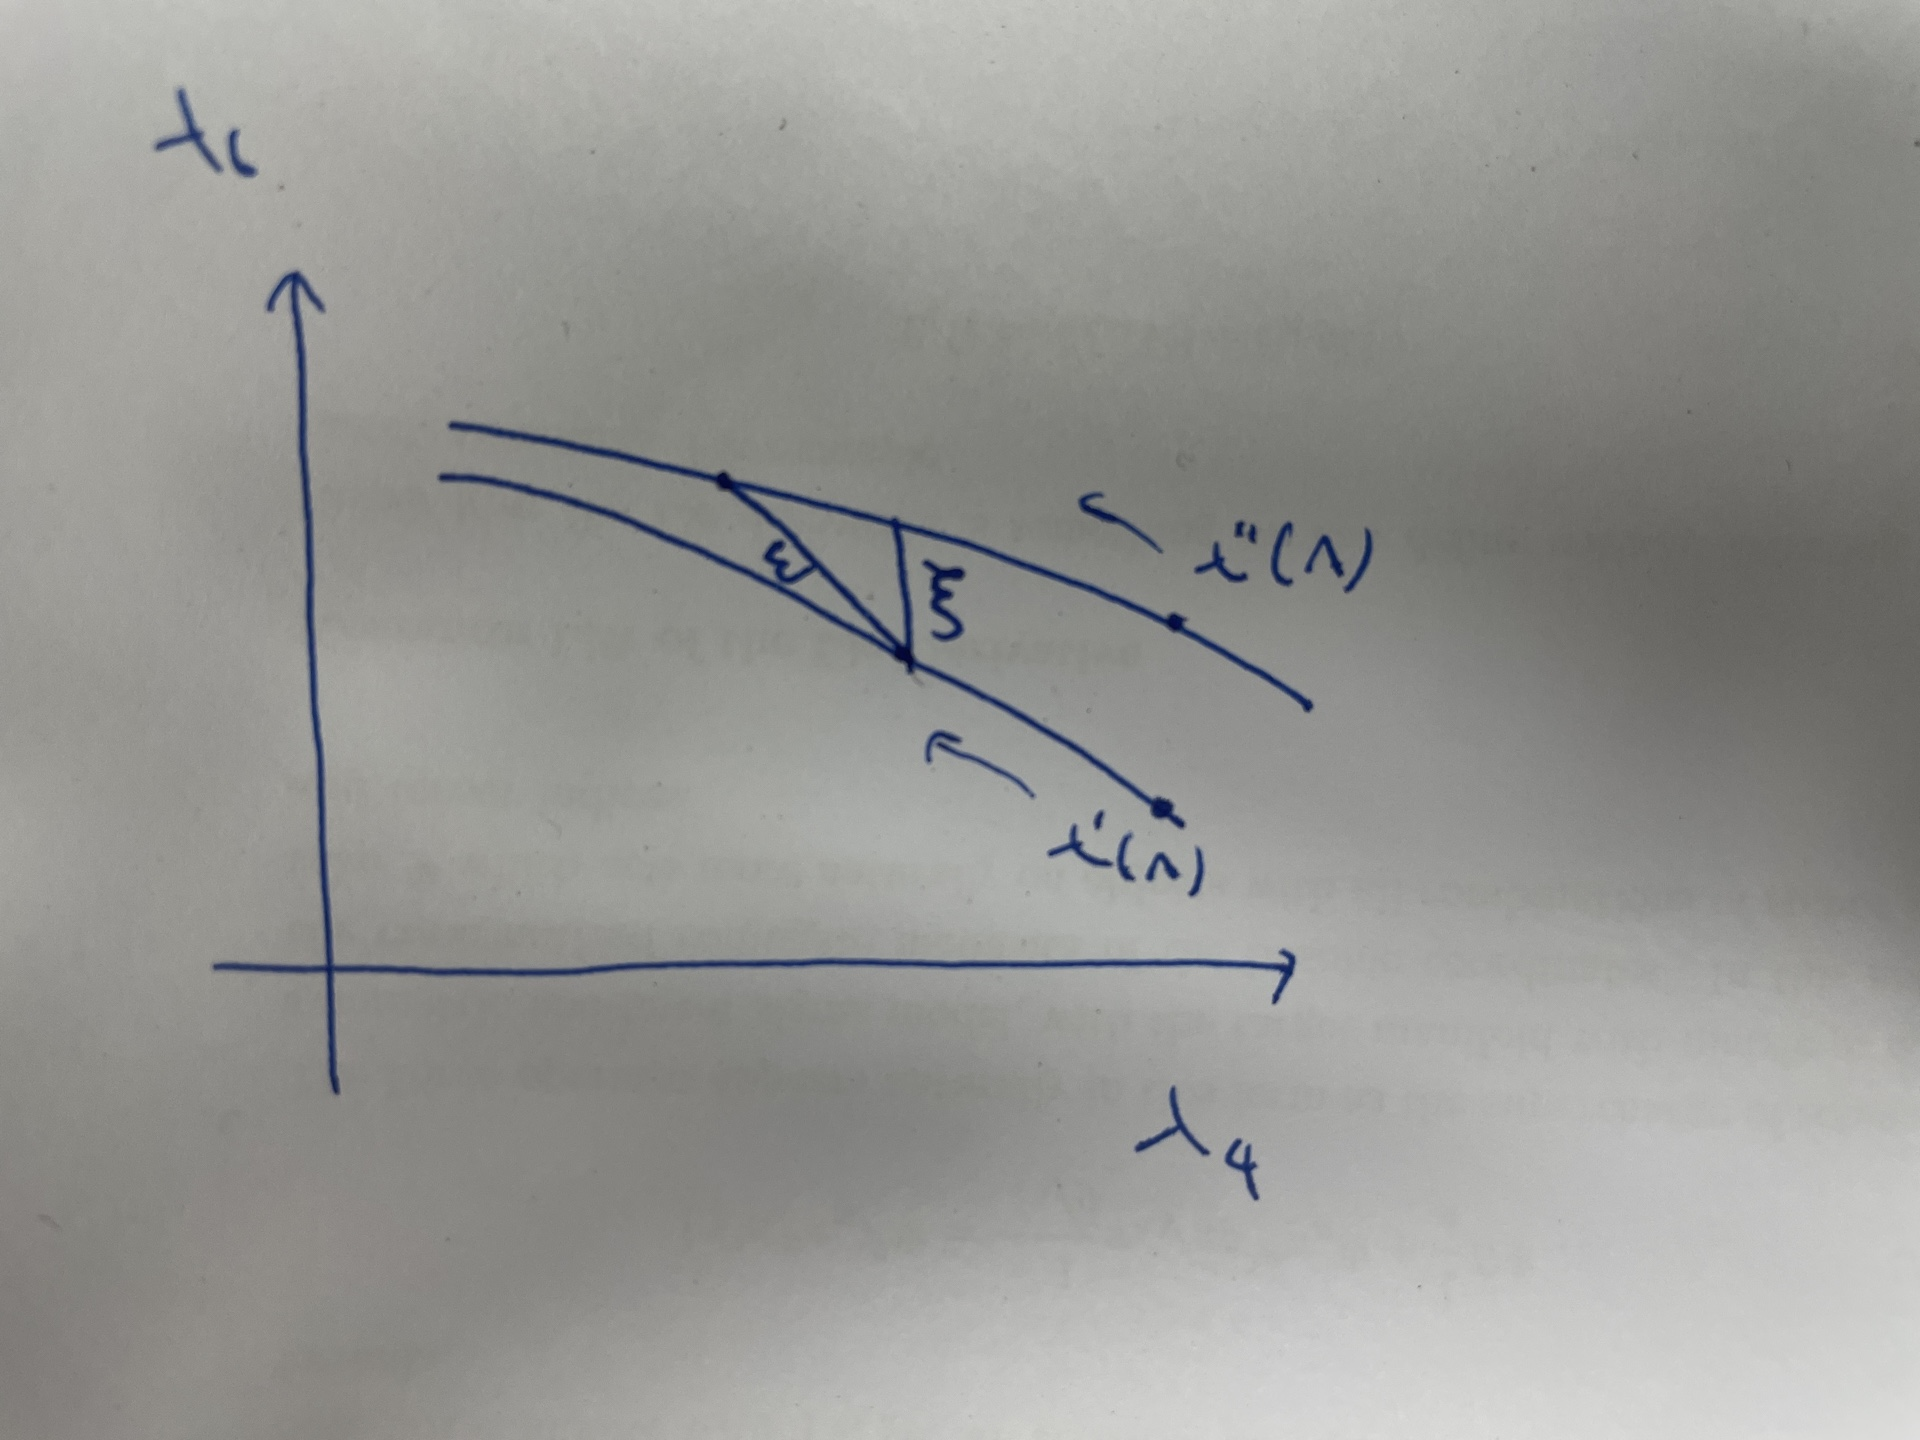
\includegraphics[width=0.7\textwidth]{Fig1.jpeg}
	\caption{RG flow in 2D parameter space}
	\label{fig:RGflow}
\end{figure}
This correspond to back-track the further evolution of $\lambda^{\prime\prime}$, and take the point directly above the point in $\lambda^\prime$, get the distance in $i$ direction.
This situation is graphically discribed in the figure \ref{fig:RGflow}.

	
Take a derivative on $\xi_6$ with respect to $\ln\Lambda$ and some substitution, we can get
\begin{equation}
	\label{eq:xi6}
	\frac{d\xi_6}{d\ln\Lambda}-2\xi_6=\bigg(\frac{\partial\beta_4}{\partial\lambda_4}+\frac{\partial\beta_6}{\partial\lambda_6}-\frac{d\ln\beta_4}{d\ln\Lambda}\bigg)\bigg\lvert_{\lambda^\prime}\xi_6
\end{equation}
Can be integrated to
\begin{equation}
	\xi_6(\mu) = \xi_6(\Lambda)\bigg(\frac{\mu^2}{\Lambda^2}\bigg)\bigg(\frac{\beta_4(\Lambda(\mu))}{\beta_4(\Lambda_0)}\bigg)\exp\int^\mu_\lambda dE\frac{1}{E}\bigg(\frac{\partial\beta_4}{\partial\lambda_4}+\frac{\partial\beta_6}{\partial\lambda_6}\bigg)\bigg\lvert_{\lambda^\prime}
\end{equation}
Thus this value is suppressed by inverse square power of $\Lambda$ in IR region, As expected.

Let us summarize the conclusion of the argument on this toy model. Let us have bare coupling $\lambda_4^\Lambda$ and $\lambda_6^\Lambda$, at scale $\Lambda$. this theory flows through the parameter space according to the RG flow,
to the thin manifold, has width of $\Lambda^{-2}$. if we take this cutoff to the infinity, it will reaches the limit. This is the handy argument that rephrase the term ``Renormalizability" in the language of RG flow.

For further use, we'll take a some note and additional discription on mathematical object here.
In the spirit of coarse-graining, renormalization is always downwards, but it is possible to define the bare lagrangian from effective lagrangian at lower scale $\mu$.
For example, consider we have the effective lagrangian $\mathcal{L}_\mu$, with renormalized coupling $\lambda_4^\mu$. the back-track the RG flow to the scale of $\Lambda$,
We'll get the bare couplings. Hence we can define the bare coupling implicitly by function of renomalized coupling, lower and upper energy scale, $\mu$, $\Lambda$, respectively.
Or vice versa, as we known as before. Former can be written as $\lambda^R(\mu,\Lambda,\lambda^\Lambda)$, while latter can be written as $\lambda^\Lambda(\mu,\Lambda,\lambda^R)$. It is helpful to think RG flow as `string' connect the two (effectively) equivalent lagrangian. The each end-points of the string is parametrized by $\mu$ and $\Lambda$ that connects the two lagrangians.
Of course they are not independent. Thus, a derivative like

\begin{equation}
	\frac{\partial}{\partial \lambda_4^\Lambda}\lambda_i(\mu,\Lambda,\lambda_i^\Lambda)
\end{equation}
This means that rate of change of renormalized coupling at scale $\mu$ with respect to the bare coupling at scale $\Lambda$.
Another example is 
\begin{equation}
	\frac{\partial}{\partial \ln\Lambda}\lambda_i(\mu,\Lambda,\lambda_i^\Lambda)
\end{equation}
means that if the bare lagrangian at scale $\Lambda$ is in fact at different scale, represents how does the renormalized coupling at scale $\mu$ changes.

\section{Polchinski's RG equation}
It is also worth that how Polchinski implement the renormalization, integration of partial mode, differentely from Heat Kernel method that we used in class.
First, write the usual path integral with the source term,
\begin{equation}
	\mathcal Z[j]=\int\mathcal D \phi e^{-S_E+J\circ\phi}
\end{equation}
Where the action $S_E$ is written in momentum basis with the interaction lagrangian
\begin{equation}
	-S_E=\int \frac{d^4p}{(2\pi)^4}\big[-\frac{1}{2}\phi(p)\bigg(\frac{1}{p^2+m^2}\bigg)^{-1}\phi(-p)+J(p)\phi(-p)\bigg]-\int d^4x \mathcal L_\text{int}
\end{equation}
Now this is the key point. Polchinski introduce the cutoff function $K(p/\mu)$ on the propagator, which satisfy the following properties
\begin{align}\begin{split}
	&\left\{
	\begin{aligned}
		&K(p/\mu)=1\quad\text{for}\quad |p|\ll\mu\\
		&K(p/\mu)=0\quad\text{for}\quad |p|\gg\mu
	\end{aligned}
	\right.
\end{split}\end{align}
and also similar properties for the source term $J(p)$.
Cutoff function is rapidly decresing around $|p|~\mu$ like a heavyside step function. But step function is not differentiable, several other options can be considered.
In Polchinski's case, he uses
\begin{align}\begin{split}
	&\left\{
		\begin{aligned}
	K(p/\mu)&=1\quad \text{for} \quad p^2\leq\mu^2\\
	K(p/\mu)&=\exp\big(\frac{e^{(4-p^2/\mu^2)^{-1}}}{1-p^2/\mu^2}\big)\quad \text{for} \quad \mu^2<p^2<4\mu^2\\
	K(p/\mu)&=0\quad \text{for} \quad p^2\geq 4\mu^2\\
\end{aligned}
\right.
\end{split}\end{align}
But after check the shape of the function, maybe there is the mistake here. This cutoff function will implement the coarse-graining. The reason why this can happen will be more clear in the next chapter, but for now just accept this fact. The path integral changes to
\begin{equation}
	-S_E=\int \frac{d^4p}{(2\pi)^4}\big[-\frac{1}{2}\phi(p)\bigg(\frac{K(p^2/\mu^2)}{(p^2+m^2)}\bigg)^{-1}\phi(-p)+J(p)\phi(-p)\big]-\int d^4x \mathcal L_\text{int}
\end{equation}
Partition function should be independent of cutoff $\mu$, thus following condition should be satisfied
\begin{align}\begin{split}
	\label{eq:floweq}
	&\frac{d}{d\ln\mu}\mathcal Z[j]=0\\
	&=\int\mathcal D \phi e^{-S_E+J\circ\phi}\bigg[-\frac{1}{2}\phi(p)\bigg(\frac{1}{(p^2+m^2)}\bigg)^{-1}\phi(-p)\frac{\partial K^{-1}}{\partial\ln \mu}+\frac{d \mathcal L}{d\ln \mu}\bigg]
\end{split}\end{align}
Where subscript int on interaction lagrangian is omitted for simplicity. We'll not denote this subscript further. 

We can already feel the traces of the Callan-Symanzik equation here. 
Let's simply replace the full differential with a partial differential, and let the parameters describing the Lagrangian be described by $\lambda_i$. 
\begin{equation}
\bigg(\frac{\partial }{\partial \ln \mu}+\frac{\partial \lambda_i}{\partial \ln \mu}\frac{\partial}{\partial \lambda_i}\bigg)\mathcal Z=0
\end{equation}
It's slightly different in subject and form from the more commonly recognized Callan-Symanzik, but you can see the connection.

Suppose following Polchinski's ansatz
\begin{equation}
	\label{eq:polchinski}
	\frac{d\mathcal L}{d\ln\mu}=-\frac{1}{2}\int d^4p\frac{(2\pi)^4}{p^2+m^2}\frac{\partial K}{\partial \ln\mu}\bigg[\frac{\delta \mathcal L}{\delta \phi(-p)}\frac{\delta \mathcal L}{\delta \phi(p)}+\frac{\delta^2 \mathcal L}{\delta \phi(p)\delta \phi(-p)}\bigg]
\end{equation}
As well as cutoff on the propagator, just accept this equation as nice ansatz for now. substitue \ref{eq:polchinski} into \ref{eq:floweq}, we get
\begin{equation}
	\label{eq:floweq2}
	\frac{dZ}{d\ln \mu} = \int d^4p \frac{\partial K}{\partial\ln \mu}\int \mathcal D \phi\frac{\delta}{\delta \phi(p)}\bigg(\phi(p)K^{-1}+\frac{(2\pi)^4}{p^2+m^2}\frac{\delta}{\delta\phi(-p)}\bigg)e^{-S_E+J\circ\phi}
\end{equation}
if the rightmost derivation of $\delta/\delta\phi(-p)$ is acted on interaction part $\mathcal L$ in the $e^{-S_E}$ and react again with $\delta/\delta\phi(p)$ at the left, it will generate the terms that related with \ref{eq:polchinski},
the remainining part of \ref{eq:floweq} is generated by $\delta/\delta\phi(p)$ acting on the propagator. $(p^2+m^2)/(K^{-1})$ term will dragged down and create the $\partial K^{-1}/\partial \ln \mu$ term by multiplied with $\partial K/\partial \ln \mu$ and $K^{-1}$.
There will additional term, dragged down soruce term $J$ by $\delta/\delta\phi(p)$ and sole $K^{-1}$ term, but the $\int d^4p \partial_{\ln \mu} K$ at the front has no overlap with these two terms therefore RHS of \ref{eq:floweq2} is equivalently same as \ref{eq:floweq}.

Now the second integral is the integral of functional derivative, same as a boundary term, goes to zero. Hence the implenting the cutoff function on the propagator, if the effective lagrangian changes according to the \ref{eq:polchinski}, the physics described by lagrangian is equivalently same.

\section{Diagrammatic expression of RG}
\label{sec3}
One might suspicious about why all this things happen. To things to be more clear, it is helpful to understand how wilsonian RG is performed in perturbative sense, using friendly tool,
the Feynmann Diagram.
Let's start again with the scalar theory. We can write the effective action as
\begin{equation}
	\label{eq:partialint}
\int \mathcal D \phi e^{-S_E^\Lambda}=\int \mathcal D \phi_> \int \mathcal D \phi_< e^{-\Delta S_E^\Lambda}=\int \mathcal D \phi_< e^{-S_E^{\Lambda}-\Delta W}
\end{equation}
where $S_E^\Lambda+\Delta W$ became effective action $S_E^\mu$ as usual, and $\phi_>$ and $\phi_<$ are the field modes with momentum greater and less than $\mu$, respectively.
One important thing to notice is $\Delta W$ can be written in terms of correlation function. Write the lagrangian in seperated manner,
\begin{equation}
	\mathcal L=\frac{1}{2}\partial_\mu\phi\partial^\mu\phi +\frac{1}{2}m^2\phi^2 +\mathcal L_{\text{int}}=\frac{1}{2}\partial_\mu\phi\partial^\mu\phi +\frac{1}{2}m^2\phi^2 + g_4\phi^4 
\end{equation}
or 
\begin{equation}
	S_E = \int d^4x \mathcal L = S_\text{free}+V_\text{int}
\end{equation}
Now applying background field method $\phi=\phi_>+\phi_<$ and working in fourier basis, the free part of the action is completely seperable
\begin{equation}
	\label{eq:sepaction}
	S_0 = \frac{1}{2}\int^\mu \frac{d^4p}{(2\pi)^4}\phi_<(-p)(p^2+m^2)\phi_<(p)+\frac{1}{2}\int^\Lambda_\mu \frac{d^4p}{(2\pi)^4}\phi_>(-p)(p^2+m^2)\phi_>(p)
\end{equation}
But the many cross terms in interaction part. so let them write $V_\text{int}[\phi_>,\phi_<]$
Then path integral of \ref{eq:partialint} can be written as
\begin{equation}
	\int \mathcal D \phi_<\int \mathcal D \phi_> e^{-S_\text{free}}e^{-V_\text{int}[\phi_>,\phi_<]}\sim\int \mathcal D \phi_< e^{-S_\text{free}[\phi_<]}\langle e^{-V_\text{int}[\phi_<]}\rangle_>
	\end{equation}
Where $\langle e^{-V_\text{int}[\phi_<]}\rangle_>$ is the average of the interaction part with respect to the field modes with momentum greater than $\mu$, says
\begin{equation}
	\label{eq:largeexpectation}
	\langle\mathcal O \rangle_> = \frac{\int \mathcal D \phi_>\mathcal O e^{-S_\text{free}[\phi_>]}}{\int \mathcal D \phi_> e^{-S_\text{free}[\phi_>]}}
\end{equation}
Up to this point, nothing is different from background field method what we did in class. But difference enters here. Since $\langle e^{-V_\text{int}} \rangle_> =\exp(\ln\langle e^{-V_\text{int}} \rangle_>)$, $\Delta W$ will contributes to the effective action as in the forms of $-\ln\langle e^{-V_\text{int}}\rangle$.
But in perturbative sense, the value $\langle \mathcal O \rangle$ can be nicely written in terms of $n$-point correlation functions. 

It is worth mention that more general statements. If we keep interaction term $V_\text{int}$ small, we can write, with use of the symbol $\langle\cdot\rangle_0$ as the expectation value of the free part of the action,
\begin{equation}
	\langle\mathcal O \rangle_0 = \frac{\int \mathcal D \phi\mathcal O e^{-S_\text{free}}}{\int \mathcal D \phi e^{-S_\text{free}}}
\end{equation}
Then we can write the expectation value in the presence of interaction term as, in terms of $n$-point correlation function, with free expectation value
\begin{align}\begin{split}
	\label{eq:perturbative}
	\langle \mathcal O \rangle &= \frac{\int \mathcal D \phi \mathcal O e^{-S_\text{free}-V_\text{int}}}{\int \mathcal D \phi e^{-S_\text{free}-V_\text{int}}}=\frac{\int \mathcal D \phi \mathcal O e^{-S_\text{free}}[1-V_\text{int}+\frac{1}{2}V_\text{int}^2-...]}{\int \mathcal D \phi e^{-S_\text{free}}[1-V_\text{int}+\frac{1}{2}V_\text{int}^2-...]}\\
	&=\frac{\langle \mathcal O \rangle_0 -\langle \mathcal O V_\text{int} \rangle_0 +\frac{1}{2}\langle \mathcal O V_\text{int}^2 \rangle_0-...}{1 -\langle V_\text{int} \rangle_0 +\frac{1}{2}\langle V_\text{int}^2 \rangle_0-...}\\
	&=(\langle \mathcal O \rangle_0 -\langle \mathcal O V_\text{int} \rangle_0 +\frac{1}{2}\langle \mathcal O V_\text{int}^2 \rangle_0-...)(1+\langle V_\text{int} \rangle_0+\langle V_\text{int} \rangle_0^2 -\frac{1}{2}\langle V_\text{int}^2 \rangle_0-...)+...
\end{split}\end{align}
where the power series expansion of $(1+x)^{-1}$ is used for last line. Collecting the terms in respect to order of operators, then the result will be
\begin{align}
	\begin{split}
\langle\mathcal O \rangle &= \langle \mathcal O \rangle_0 - (\langle\mathcal O V_\text{int}\rangle_0-\langle\mathcal O\rangle_0\langle V_\text{int}\rangle_0)\\
&+\frac{1}{2}(\langle \mathcal O V_\text{int}^2 \rangle_0-2\langle \mathcal O V_\text{int} \rangle_0\langle V_\text{int} \rangle_0+2\langle \mathcal O \rangle_0\langle V_\text{int} \rangle_0^2-\langle \mathcal O \rangle_0\langle V_\text{int} \rangle_0^2)\\
&+...
	\end{split}
\end{align}
without the proof, this result generalized to all order as 
\begin{equation}
	\langle\mathcal O\rangle_0 = \sum^\infty_{n=0}\frac{-1^n}{n!}\langle \mathcal O V_\text{int}^n\rangle_0^c
\end{equation}
in terms of `connected averages'
  in terms of feynman diagram, the unconnected diagram will be cancelled each other while calculating $\langle\mathcal O V_\text{int}^n\rangle_0^c$. This is the same statement as $n$-point correlation function is calculated by $n$-external leg diagram, without the contributions from the disconnected diagrams. this is called \textbf{Linked Cluster Theorem}.

now turn back to the our scalar field theory. We have to calculate $-\ln\langle e^{-V_\text{int}}\rangle_>$ perturbatively. Again, write perturbative expansion of
\begin{equation}
	\langle e^{-V_\text{int}}\rangle_> \sim 1-\langle V_\text{int}\rangle_>+\frac{1}{2}\langle V_\text{int}^2\rangle_> ...
\end{equation}
then use taylor expansion of $\ln(1+x)\sim x-x^2/2$ up to $\mathcal O (V_\text{int}^2)$
\begin{align}
	\begin{split}
	\ln\langle e^{-V_\text{int}}\rangle_> &=-\langle V_\text{int}\rangle_> +\frac{1}{2}\langle V_\text{int}^2\rangle_>-\frac{1}{2}(-\langle V_\text{int}\rangle_>+\frac{1}{2}\langle V_\text{int}^2\rangle_>)^2+\mathcal O(V_\text{int}^2)\\
	&=-\langle V_\text{int}\rangle_>+\frac{1}{2}(\langle V_\text{int}^2\rangle_> - \langle V_\text{int}\rangle_>^2)
	\end{split}
\end{align}
Therfore, at least perturbatively, the action changes by
\begin{align}
	\begin{split}
		\int\mathcal D\phi e^{-S_E}\rightarrow \#\int\mathcal D\phi_<e^{-S_E-\langle V_\text{int}\rangle_>+\frac{1}{2}(\langle V_\text{int}^2\rangle_> - \langle V_\text{int}\rangle_>^2)} 
	\end{split}
\end{align}
Or, says,
\begin{equation}
	-\Delta W = -\langle V_\text{int}\rangle_>+\frac{1}{2}(\langle V_\text{int}^2\rangle_> - \langle V_\text{int}\rangle_>^2)
\end{equation}
This is the most important parts. Recall that how we make the feynman diagram. Since we're working with the $\phi^4$ theory, which generate the $V_\text{int}$ as the mixing of $\phi_>$ and $\phi_<$ with order 4.
Since we coarse-graining the $\phi_>$, by embrace the $\langle \cdot \rangle_>$ sign, then by the Wick's theorem, the $\phi_>$ leg will be connected each other, an will integrated out. Let's see this with the explicit diagrammatic expression.

Before that, let's write the $V_\text{int}$ in fourier basis.
\begin{align}
	\begin{split}
		V_\text{int} &= g_4\int d^4x \phi^4 
		\\&= g_4\int \frac{d^4p_1}{(2\pi)^4}\frac{d^4p_2}{(2\pi)^4}\frac{d^4p_3}{(2\pi)^4}\frac{d^4p_4}{(2\pi)^4}\phi(p_1)\phi(p_2)\phi(p_3)\phi(p_4)\int d^4x e^{i(p_1+p_2+p_3+p_4)^\mu x_\mu}\\
		&=g_4\int(2\pi)^4\delta(p_1+...+p_4)\prod_{i=1}^4\frac{d^4p_i}{(2\pi)^4}(\phi(p_i)_<+\phi(p_i)_>)
	\end{split}
\end{align}
Which will creat the 5 different kind of terms characterize by different number of $\phi_>$ included between total 4 $\phi$'s, while their coeffcients will determined by the ${4\choose n}$.
\subsection{$\langle V_\text{int} \rangle_>$ contribution.} 
\begin{figure}[ht]
	\centering
	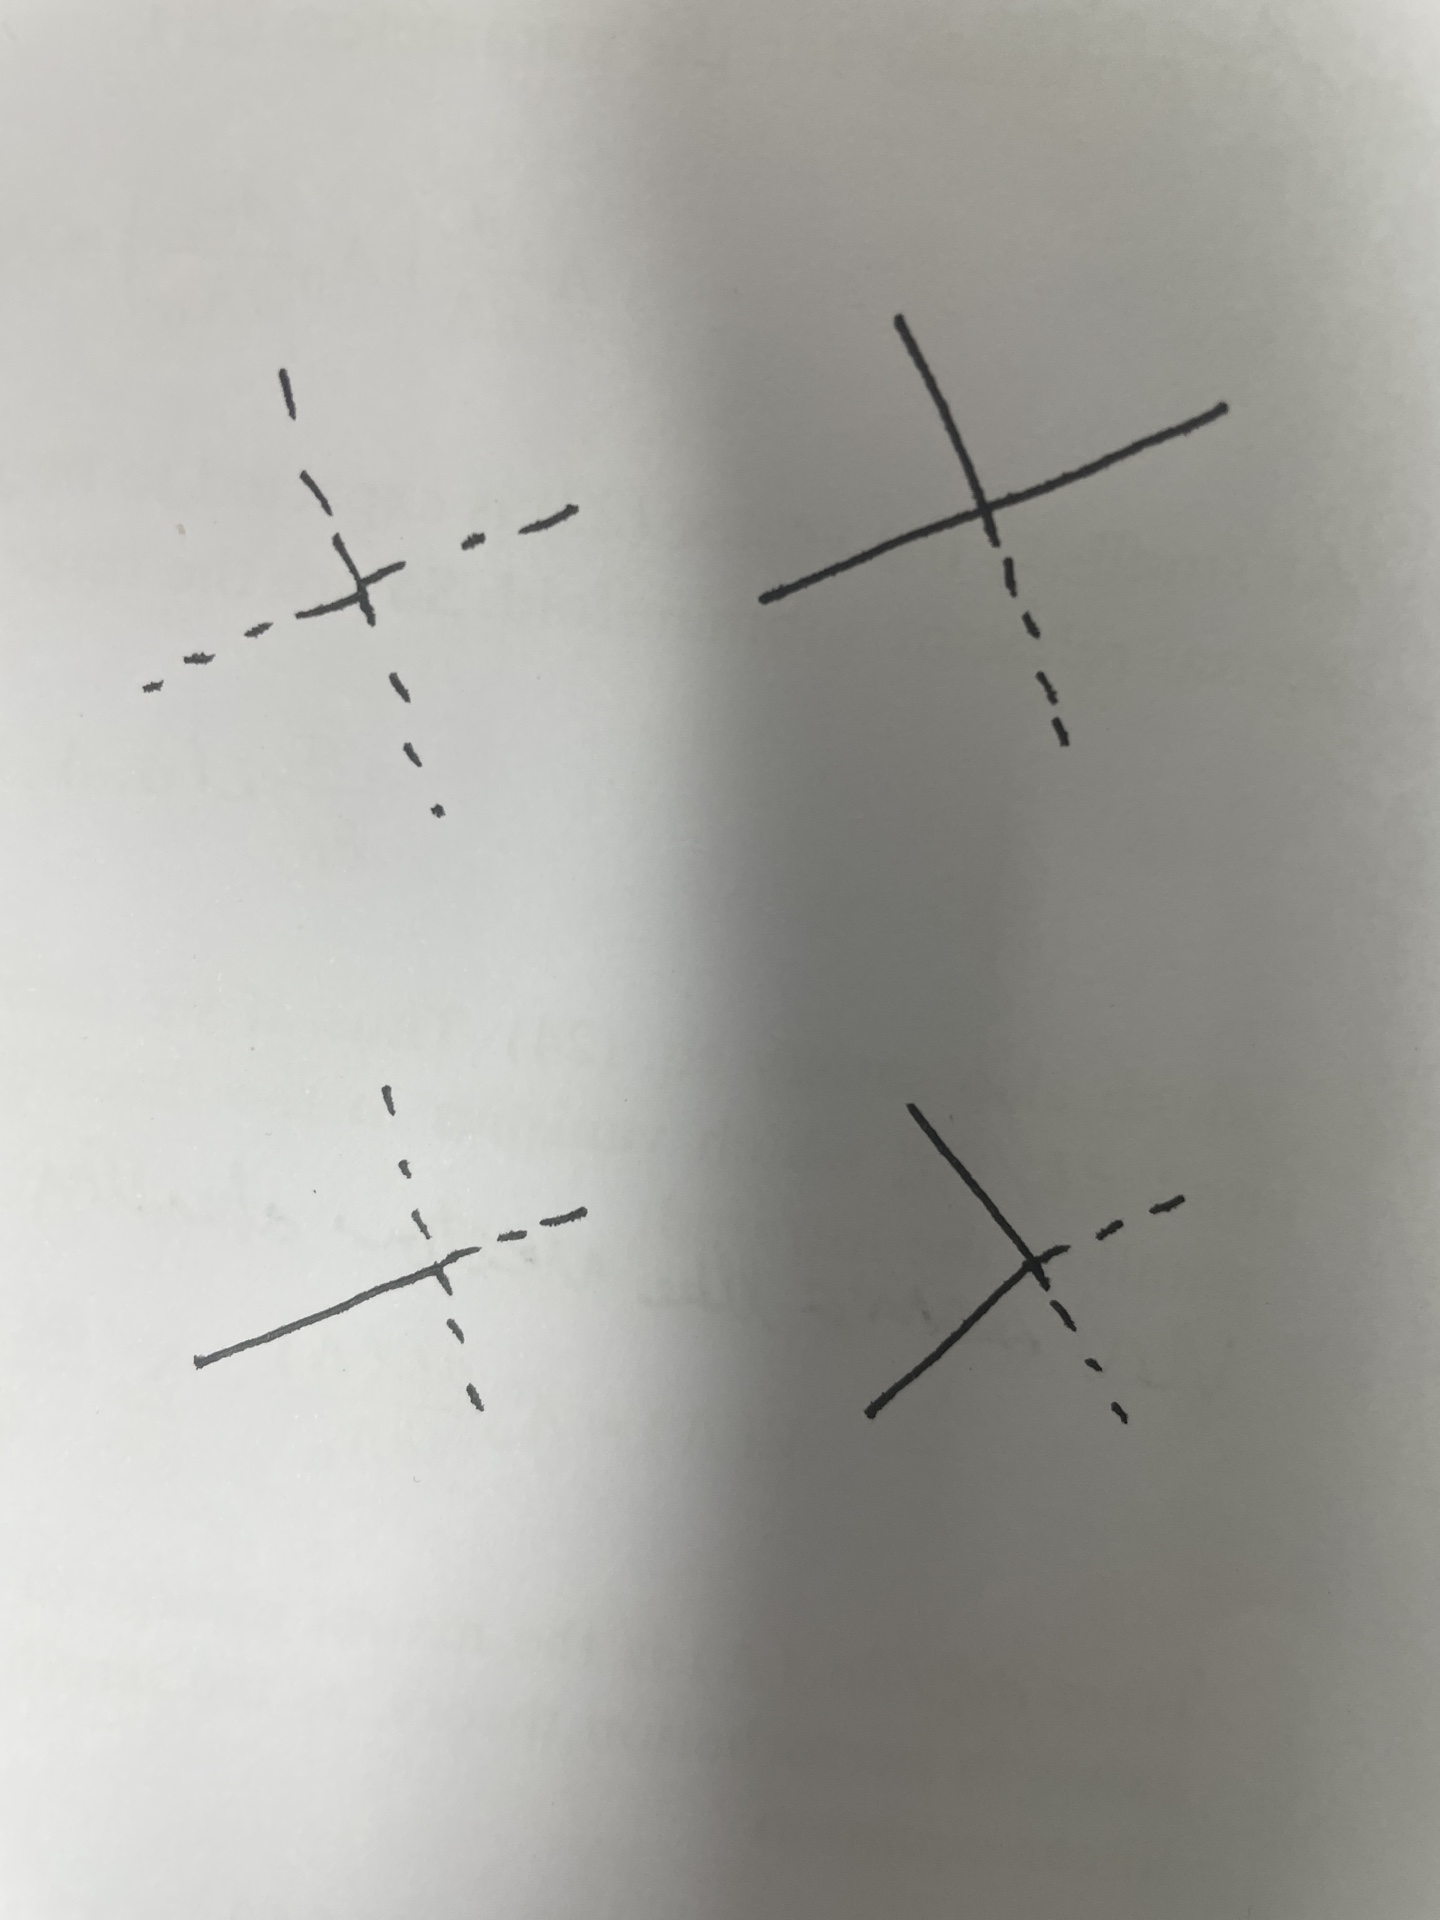
\includegraphics[width=0.4\textwidth]{Fig2.jpeg}
	\caption{Different kind of $V_\text{int}$. $\phi_>$ is noted by the dashed line.} 
	\label{fig:Vsing}
\end{figure}
First compute the simple case, $\langle V_\text{int} \rangle_>$. $V_\text{int}$ can be categorized by the number of $\phi_>$, like the figure \ref{fig:Vsing}.
After applying $\langle \cdot \rangle_>$, the $\phi_>$ will be connected each other by wick's theorem, and will be integrated out.
It is straightforward that terms that odd(in this case, 1 or 3) number of $\phi_>$ will be vanished.
Let's see what will happen on terms that have two $\phi_>$.
only way to contract two dashed line is described in the figure \ref{fig:Vdouble}. Right part have two external leg with $\phi<$. As we can see, vertex changes effectively to mass term!

\begin{figure}
	\centering
	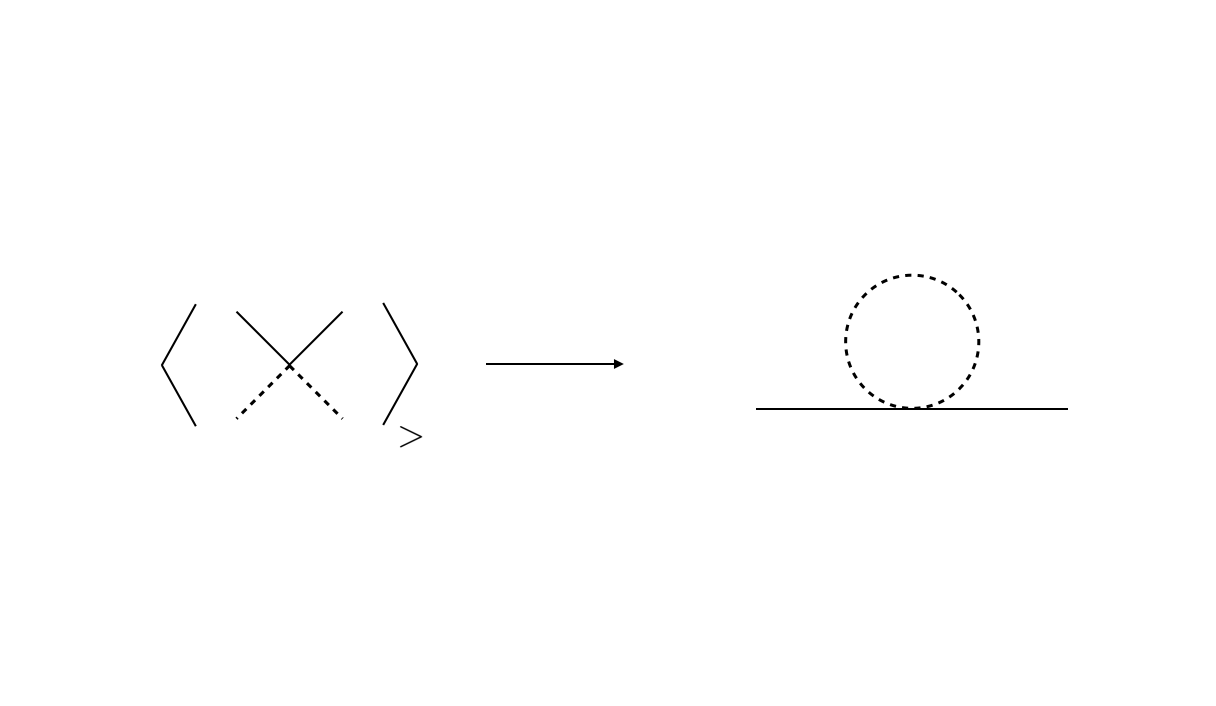
\includegraphics[width=0.4\textwidth]{Fig3.jpeg}
	\caption{The only way to contract two $\phi_>$ in $V_\text{int}$.}
	\label{fig:Vdouble}
\end{figure}
If write this as a formula, the story goes same. the left side of the figure \ref{fig:Vdouble} is
\begin{equation}
		g_4\int(2\pi)^4\delta(p_1+...+p_4)\phi(p_1)_<\phi(p_2)_<\phi(p_3)_>\phi(p_4)_>\prod_{i=1}^4\frac{d^4p_i}{(2\pi)^4}
\end{equation}
embracing the $\langle \cdot \rangle_>$, means
\begin{align}
\begin{split}
\label{eq:massshiftcalc}
	&g_4\int(2\pi)^4\delta(p_1+...+p_4)(\phi(p_1)_<\phi(p_2)_<)\langle\phi(p_3)_>\phi(p_4)_>\rangle_>\prod_{i=1}^4\frac{d^4p_i}{(2\pi)^4}\\
=&g_4\int(2\pi)^4\delta(p_1+...+p_4)(\phi(p_1)_<\phi(p_2)_<)\frac{(2\pi)^4\delta^4(p_3+p_4)}{m^2+p_3^2}\prod_{i=1}^4\frac{d^4p_i}{(2\pi)^4}\\
=&g_4(2\pi)^4\int^\mu\delta(p_1+...+p_4)\frac{d^4p_1}{(2\pi)^4}\frac{d^4p_2}{(2\pi)^4}(\phi(p_1)_<\phi(p_2)_<)\times\\
&\int_\mu^\Lambda\frac{(2\pi)^4\delta^4(p_3+p_4)}{m^2+p_3^2}\frac{d^4p_4}{(2\pi)^4}\frac{d^4p_3}{(2\pi)^4}\\
&=g_4\int^\mu\bigg[\frac{d^4p}{(2\pi)^4}\phi(-p)_<\phi(p)_<\bigg]\int^\Lambda_\mu\frac{d^4k}{(2\pi)^4}\frac{1}{m^2+k^2}	
\end{split}
\end{align}
Because the two-point correlation function is the propagator(actually, this argument is logically preceding than diagrammatic expression). The term inside $[\cdot]$ has same form as mass term in effective action, thus thus diagram contributes to the mass term in the effective action.
Numerical factor is ${4\choose 2}$(due to exapnsion)$\times 1$($\#$way of wick contraction) = 6, thus
\begin{equation}
	\frac{1}{2}m^2\rightarrow\frac{1}{2} m^2+\frac{6g_4}{(2\pi)^4}\int^\Lambda_\mu\frac{d^4k}{m^2+k^2}
\end{equation}
This is the only thing we have to consider, because other case will be vanished by odd-contraction rule off wick contraction or it contributes up to the constant factor.
\subsection {$\frac{1}{2}(\langle V^2_\text{int} \rangle-\langle V_\text{int} \rangle^2)$ contribution.}
\label{sec:v2}
For second order on $V_\text{int}$, calculation will be lengthy, but the idea is the same. Two 4-legs vertex, contraction between $\phi_>$.
\begin{figure}[h!]
	\centering
	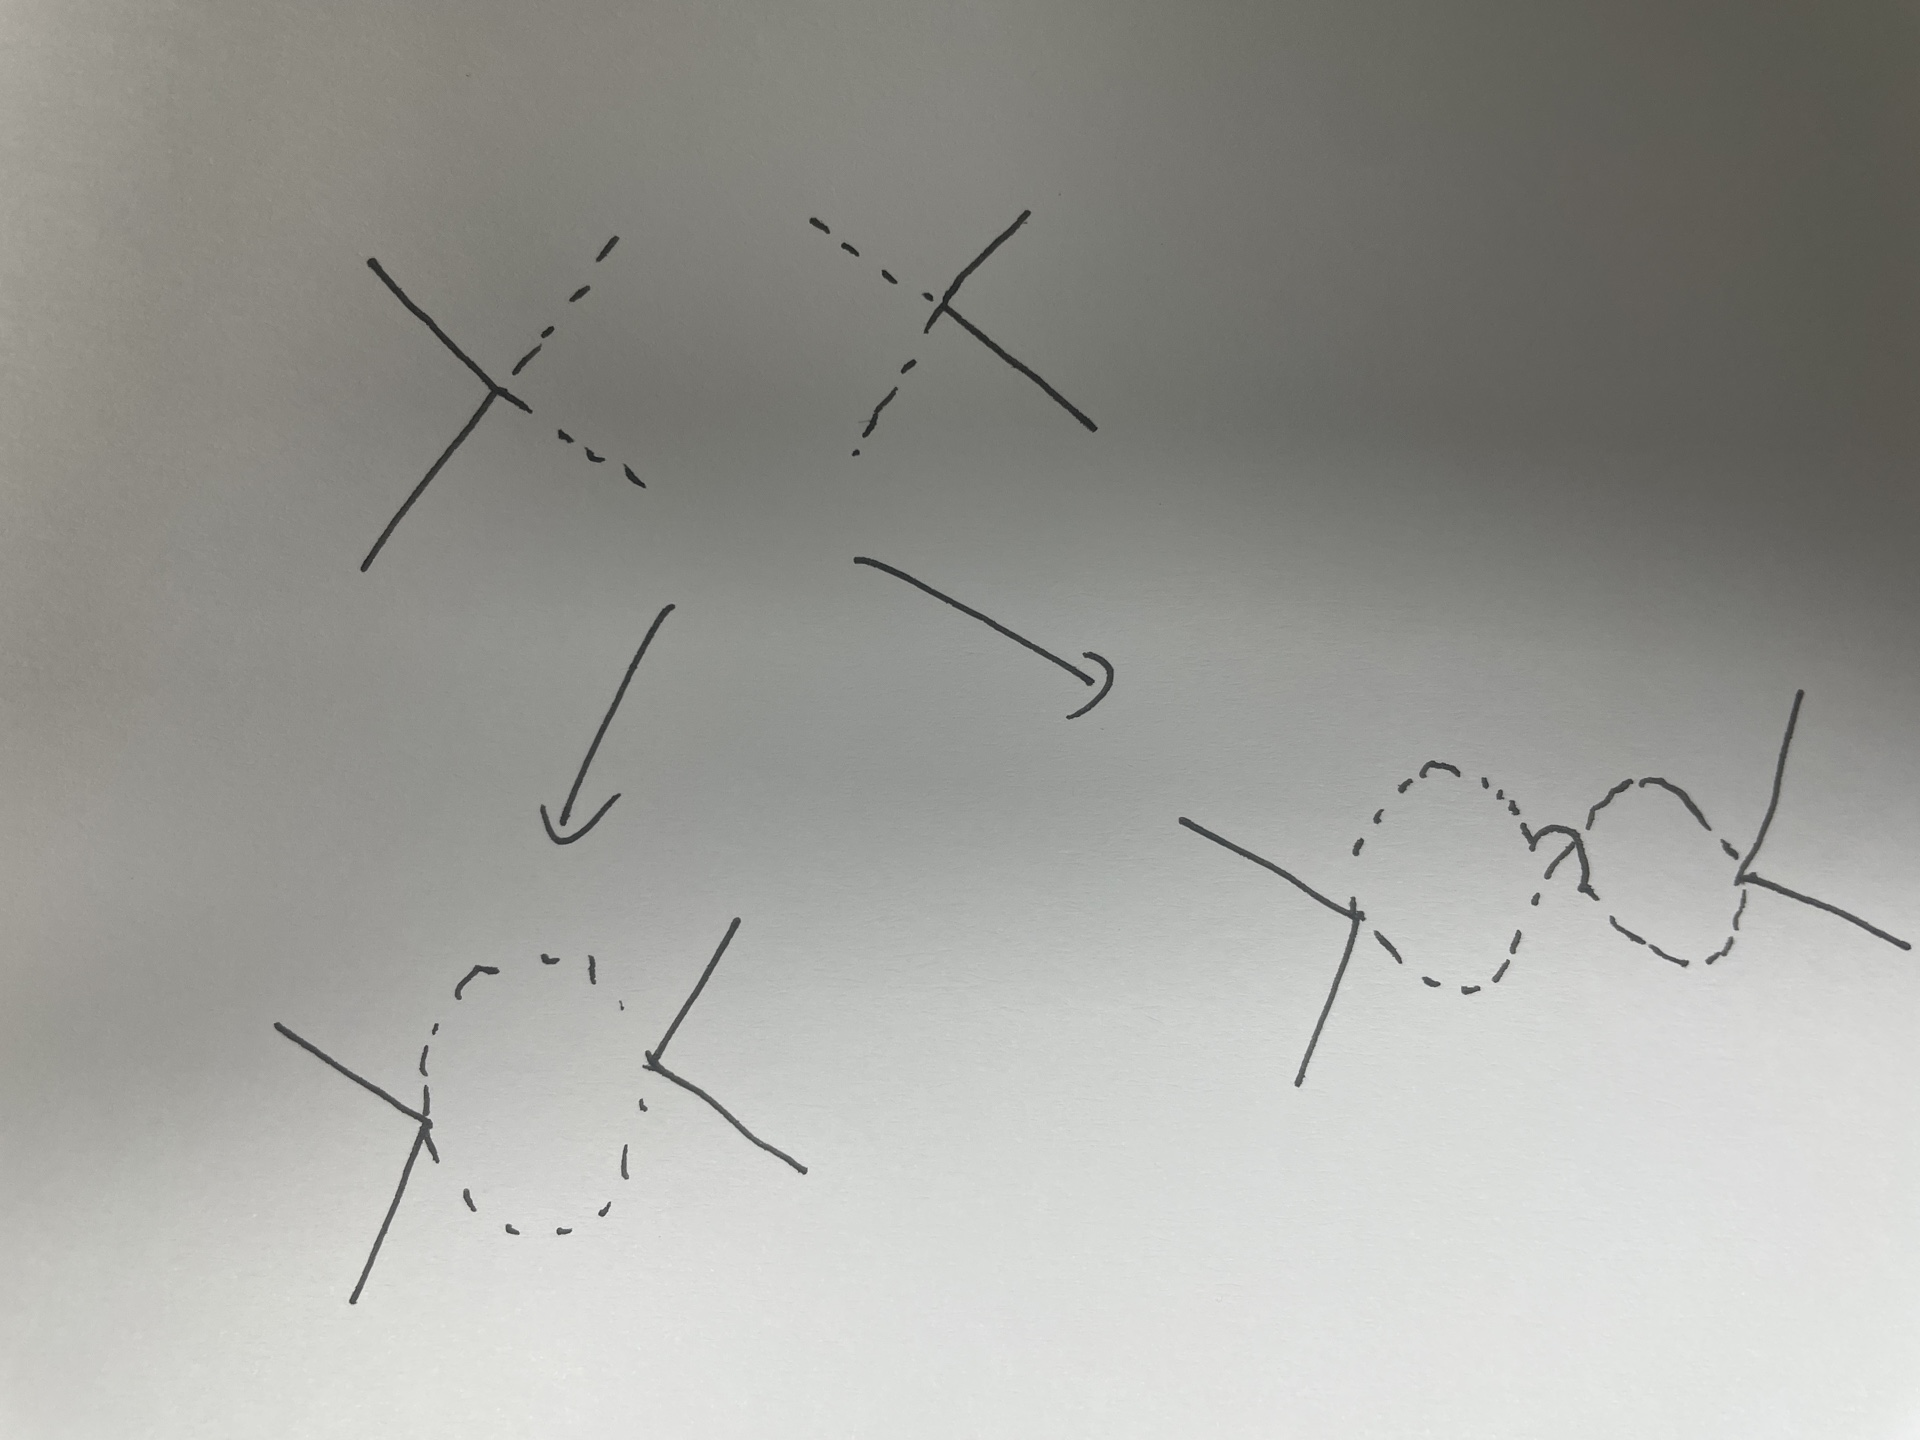
\includegraphics[width=0.4\textwidth]{Fig4.jpeg}
	\caption{The only way to contract two $\phi_>$ in $V_\text{int}$.}
	\label{fig:Vdoubledouble}
\end{figure}
Figure \ref{fig:Vdoubledouble} shows the two possible way to contract two $\mathcal{O}(\phi_<^2\phi_>^2)$ term. Of course their functional form should be same, but there are addition factor generated by wick contraction, different from the Figure \ref{fig:Vdouble}.
That will be the harsh road to combinatorics and integration. However, the trenmendous simplification is done by the following reasons.
\begin{enumerate}
	\item disconnected diagram. disconnected diagram will clearly cancelled out by the $\langle V^\text{int} \rangle_>^2$ from the $\langle V_\text{int}^2 \rangle_>$ term. This is the sip of aforementioned linked cluster theorem.
	\item $\delta$ function in the vertex. consider vertex with three $\phi_>$ and $\phi_<$ vertex ans two of $\phi_>$ are contracted. Then $\delta$ function responsible for this vertex never can be non-zero. 
\end{enumerate}
For Example, the diagram in the figure \ref{fig:Vdoubledouble} has the expressed as
\begin{align}
	\begin{split}
		&g_4^2\int(2\pi)^8\delta(\sum_i^{\{1,2,5,6\}}p_i)\delta(\sum_i^{\{3,4,7,8\}}p_i)(\phi(p_1)_<...\phi(p_4)_<)\langle\phi(p_5)_>...\phi(p_8)_>\rangle_>\prod_{i=1}^8\frac{d^4p_i}{(2\pi)^4}\\
		=&2g_4^2\int(2\pi)^8\delta(\sum_i^{\{1,2,5,6\}}p_i)\delta(\sum_i^{\{3,4,7,8\}}p_i)(\phi(p_1)_<...\phi(p_4)_<)\times\\
		&\frac{(2\pi)^4\delta^8(p_5+p_7)}{m^2+p_5^2}\frac{(2\pi)^4\delta^4(p_6+p_8)}{m^2+p_6^2}\prod_{i=1}^8\frac{d^4p_i}{(2\pi)^4}\\
		=&2g_4^2\int\prod_{i=1}^4\frac{d^4p_i}{(2\pi)^4}(2\pi)^8\delta(p_1+p_2-k_1-k_2)\delta(p_3+p_4+k_1+k_2)(\phi(p_1)_<...\phi(p_4)_<)\times\\
		&\int\bigg(\prod_{i=1}^2\frac{d^4k_i}{(2\pi)^4}\bigg)\frac{1}{m^2+k_1^2}\frac{1}{m^2+k_2^2}\\
		=&2g_4^2\int\prod_{i=1}^4\frac{d^4p_i}{(2\pi)^4}(2\pi)^4\delta(p_1+p_2+p_3+p_4)(\phi(p_1)_<...\phi(p_4)_<)
		\\&\times\int\frac{d^4k}{(2\pi)^4}\frac{1}{m^2+(p_1+p_2-k)^2}\frac{1}{m^2+k^2}
	\end{split}
\end{align}
this term will contributes to $\phi_<^4$ term. Note that numerical factor of 2 is added due to multiplicity of wick contraction. The additio numerical factor is ${4\choose 2}^ 2=36$.
Hence overall factor is $-1/2\times 36 \times 2= -36$. Summarize up, by this term, effective lagrangian changes as
\begin{equation}
	g_4\rightarrow g_4-36\frac{g_4^2}{(2\pi)^4}\int^\Lambda_\mu\frac{d^4k}{(m^2+k^2)^2}
\end{equation}
With use of approximation
\begin{equation}
	\int^\Lambda_\mu\frac{d^4k}{(m^2+k^2)}\frac{1}{(m^2+(p_1+p_2-k)^2)}\sim \int^\Lambda_\mu\frac{d^4k}{(m^2+k^2)^2}
\end{equation}
\subsection{So What?-connection to Polchinski's flow equation}
So after the all messy calculation, we've seen the how lagrangian changes by coarse graining in picture of feynman diagram.
Of course this is not done by combinatorics and integration, but rather, it is done by High-mode free action, or High-mode propagator.
Recall that how things are going in previous section. At first we expand $e^{-V_\text{int}}$ in order of $V_\text{int}$(or $g_4$) at the each order of $V_\text{int}$, high mode terms contracted each other, which fully expressed by high-mode propagator,
remainins only few number of $\phi_<$ legs at the end of the day. They absorb to the low mode lagrangian then be a effective lagrangian.

Therefore, we treat the propagator in a completely seperated manner, during the coarse-graining process.
After coarse-graining is done, propagator has cutoff by process's nature, as we can check in \ref{eq:massshiftcalc} or \ref{eq:sepaction}. 
From the perspective of Wilsonian RG, giving the propagator a cutoff seems to be an approach that makes sense, but why give it to the propagator? Why is there no such requirement for interaction Lagrangians? 
In other words, this is the same approach we took in the previous “perturbative renormalization” \ref{eq:largeexpectation}. We are now looking at $V_\text{int}$ as a perturbation and doing a path integral through the high-mode free theory.

That's why it's possible to take the exact opposite approach. In the previous description, we gave a cutoff to the momentum and then integrated out the high-mode through a high-mode propagator. The result is a propagator with a cutoff, naturally. 
Here's the opposite approach I mentioned earlier: we force the propagator to give us a cutoff, but nevertheless force our partition function to remain unchanged. Of course, this requires the interaction Lagrangian to change a bit, which is Polchinski's approach, and it's safe to say that the condition on how the Lagrangian should change is Polchinski's flow equation.

More interesting than this set of intuitively easy facts is the fact that Polchinski's flow equation itself can be done exactly the same way with the Feynman diagram model we did in the previous section. Let's rewrite that expression here. 
\begin{equation}
	\label{eq:polchinski2}
	\frac{d\mathcal L}{d\mu}=-\frac{1}{2}\int d^4p\frac{(2\pi)^4}{p^2+m^2}\frac{\partial K}{\partial\mu}\bigg[\frac{\delta \mathcal L}{\delta \phi(-p)}\frac{\delta \mathcal L}{\delta \phi(p)}+\frac{\delta^2 \mathcal L}{\delta \phi(p)\delta \phi(-p)}\bigg]
\end{equation}
Replaced the $\ln$ derivative with a simple derivative only. First, notice that the derivative of the cutoff function $K$ is nonzero only just above the cutoff $\mu$, which makes intuitive sense. In the process above, we integrated the modes above the cutoff $\mu$ to generate the effective Lagrangian, so it's not surprising that the Lagrangian's variation with the cutoff $\mu$ comes out with a $\frac{\partial K}{\partial \mu}$ term that is non-zero only just above $\mu$.
It's easy to see that \ref{eq:polchinski2} also can be written as
\begin{equation}
	\frac{d\mathcal L}{d\mu}=-\frac{1}{2}\int d^4p_1d^4p_2\frac{(2\pi)^4\delta(p_1+p_2)}{p_1^2+m^2}\frac{\partial K}{\partial\mu}\bigg[\frac{\delta \mathcal L}{\delta \phi(p_1)}\frac{\delta \mathcal L}{\delta \phi(p_2)}+\frac{\delta^2 \mathcal L}{\delta \phi(p_1)\delta \phi(p_2)}\bigg]
\end{equation}
Where the $\frac{(2\pi)^4\delta(p_1+p_2)}{p_1^2+m^2}$ is doubtlessly the propagator. 
The meaning of the inner term $[\cdot]$ is now clear: each functional derivative creates a form that removes one $\phi$ from the Lagrangian. The removed $\phi$ are no different than the wick contracted ones from earlier, hence the propagators. Just as we did with the momentum shell integration, we need a suitable momentum integral range, and that is the quotient of $\frac{\partial K}{\partial \mu}$.
\begin{figure}[h!]
	\centering
	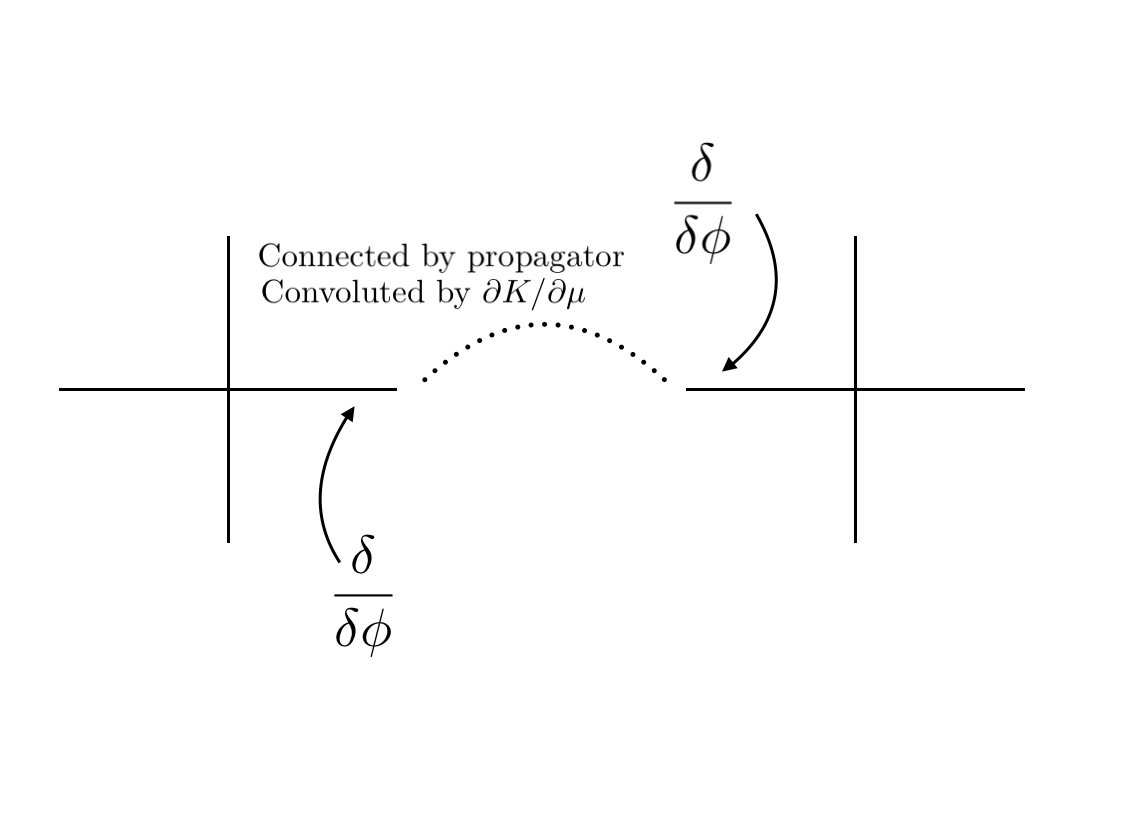
\includegraphics[width=0.6\textwidth]{Fig5.jpeg}
	\caption{The diagrammatic expression of Polchinski's flow equation. Two vertex forming tree level diagram.}
	\label{fig:polchinski}
\end{figure}

\begin{figure}[h!]
	\centering
	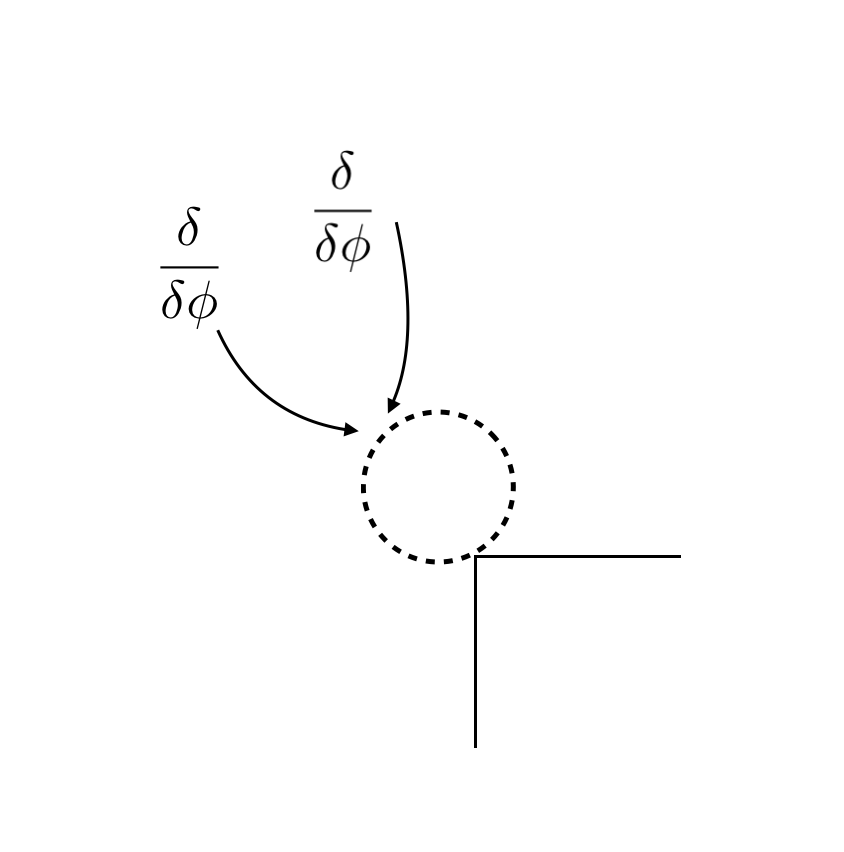
\includegraphics[width=0.6\textwidth]{Fig6.jpeg}
	\caption{One vertex forming loop diagram.}
	\label{fig:polchinski2}
\end{figure}
Now it's clear to diagram the inside of the term in $[\cdot]$. The first term picks a set of vertices in the interaction Lagrangian and picks a bridge, each of which is connected to the others to form a new vertex. The next term, on the other hand, picks two bridges from a single vertex. The two legs are connected to form a loop.

\section{Outline of Polchinski's proof of renormalizability}
But that's not the end of the story. The diagram connecting the two $\phi_<^3\phi_>$ vertices in \ref{sec:v2} implies the appearance of the $\phi^6$ operator. The second term inside $[\cdot]$ in \ref{eq:polchinski2} hints at the same message.
Of course, we know that this operator is irrelevant, so it will be small enough under certain conditions. The rest of Polchinski's paper is a mathematically rigorous proof of this from a Wilsonian point of view and with the concept of RG flow in parameter space.
We won't follow all the mathematical details of his proof here, but we'll content ourselves with picking up a few key threads and notable points.
\begin{definition}
	$\tilde{\mathcal L}(\mu,\lambda^\mu,\Lambda)$ is a effective lagrangian at energy scale $\mu$ that consists by only quartic interaction characterized by $\lambda^\mu$. They should define as cutoff $\Lambda$ and appropriate bare parameters.
\end{definition}
\begin{theorem}
	\label{thm:renormalizability}
	For a $\tilde{\mathcal L}(\mu,\lambda^\mu,\Lambda)$, it has a limit of $\Lambda\rightarrow\infty$.
\end{theorem}
To illustrate, let's consider an example where you don't have a limit. This is the Polchinsky's toy model we saw in Section \ref{sec2}, and similar to what we did earlier, we're going to linearize it, assuming beta is small, and build an expression.
\begin{align}
	\label{eq:nolimittoyexample}
	\begin{split}
		\frac{d}{d\ln \mu}\begin{pmatrix}
			\lambda_4\\\lambda_6
		\end{pmatrix}=\bigg(M+\begin{pmatrix}
			0&0\\0&2
		\end{pmatrix}\bigg)	\begin{pmatrix}
			\lambda_4\\\lambda_6
		\end{pmatrix}
	\end{split}
\end{align}

Each component of $M$ represents a derivative of beta. Assuming each component is very small, we can now diagonalize the matrix and solve the differential equation, You should get $\lambda_4(\mu)\sim~\lambda_6(\mu)\frac{\Lambda^2}{\mu^2}$ as a result.
Therefore, there is no way to leave $\lambda_6$ non-zero and eliminate the cutoff dependency of $\lambda_4$. Technically, this means no $\Lambda\rightarrow\infty$ limits.

Someone might be very suspicious of the $\Lambda\rightarrow\infty$ limit. This is because, as we know, the mass of a scalar particle has a shift corresponding to the ultraviolet cutoff $\Lambda^2$ and has no continuum limit.
However, please understand that we are not taking the extremes of $\Lambda\rightarrow\infty$ in the context of talking about continuum limits.
From the perspective of effective field theory, this is equivalent to saying that we have taken the limit of $\mu/\Lambda\rightarrow0$.


Let's start with some basic assumptions. Since we are dealing with a very complex Lagrangian that may contain many irrelevant terms generated by the flow, it is a good idea to start by defining the basic form. In fourier basis, we can write
\begin{align}
	\begin{split}
		\mathcal L(\mu) = \sum^\infty_{n=1}&\frac{1}{(2n)!}\int\prod^{2n}_{i=1}\frac{d^4p_i}{(2\pi)^4}L_{2n}(p_1,...,p_{2n},\mu)\phi(p_1)...\phi(p_{2n})\\
		&\times(2\pi)^4\delta(p_1+...+p_{2n})
	\end{split}
\end{align}
If so, the “renormalized” parameters we normally use are no different than the following
\begin{align}
	\begin{split}
		&\delta_m(\mu) = -L_2(0,0,\mu)\\
		&\delta_K(\mu) = -\frac{1}{8}\frac{\partial^2}{\partial p^2}L_2(p,-p,\mu)|_{p=0}\\
		&\lambda^\mu_4 = -L_4(0,0,0,0,\mu)
	\end{split}
\end{align}
%//TODO CHECK THIS
Each is no different than the corresponding quantities for the two-point, kinetic, and four-point terms back in real space.
%//TODO add brief description on renoramalizability

\section{Wilson, Callan-Symanzik, Conclusion}
We're almost to the conclusion. First, let's finish the discussion we had in Section \ref{sec3}.
Let's remind ourselves of how the terms have changed. 
\begin{align}
\begin{split}
	\frac{1}{2}m^2\rightarrow\frac{1}{2} m^2+\frac{6g_4}{(2\pi)^4}\int^\Lambda_\mu\frac{d^4k}{m^2+k^2}\\
	g_4\rightarrow g_4-36\frac{g_4^2}{(2\pi)^4 }\int^\Lambda_\mu\frac{d^4k}{(m^2+k^2)^2}\\
\end{split}	
\end{align}
The integral here is particularly easy to compute in the normal case where $\mu$ and $\Lambda$ much more larger than $m$. Rather than compute it right away, we'll replace it with a generalized dimension d. This is not for any particular purpose, but rather to introduce a famous concept later. So, the above expression becomes
\begin{align}
	\begin{split}
		\frac{1}{2}m^2\rightarrow\frac{1}{2} m^2+\frac{6g_4}{(2\pi)^d}\int^\Lambda_\mu dr\frac{S_{d-1}r^{d-1}}{m^2+r^2}\\
		g_4\rightarrow g_4-36\frac{g_4^2}{(2\pi)^d}\int^\Lambda_\mu dr\frac{S_{d-1}r^{d-1}}{(m^2+r^2)^2}\\
	\end{split}	
\end{align}
Here we observe the quadratic shift of the mass term as we know it (at $d=4$).


Then, we'll add a few more steps that we didn't do in class.
First, rescaling of momentum. This is a coordinate transformation rather than a process with much physical significance, but given that the spirit of coarse-graining is to observe how physics looks different at different scales,
To compare two theories at different scales, we want to equalize the momentum cutoff (rescaling might be a better way to put it - think of observing the theory as you zoom out further and further).
This can be understood as a transformation of the momentum $p^\prime=\frac{\Lambda}{\mu}p$. 
If so, it would look like this
\begin{align}
	\begin{split}
		\frac{1}{2}m^2\rightarrow\bigg(\frac{\Lambda}{\mu}\bigg)^{-d}\bigg[\frac{1}{2} m^2+\frac{6g_4}{(2\pi)^d}\int^\Lambda_\mu dr\frac{S_{d-1}r^{d-1}}{m^2+r^2}\bigg]\\
		g_4\rightarrow\bigg(\frac{\Lambda}{\mu}\bigg)^{-3d}\bigg[g_4-36\frac{g_4^2}{(2\pi)^d}\int^\Lambda_\mu dr\frac{S_{d-1}r^{d-1}}{(m^2+r^2)^2}\bigg]\\
	\end{split}	
\end{align}
Where the $S_{d-1}$ is the area of the surface area of the unit $n-1$ sphere. Each number comes from the integral measure that each term carries (You might wonder why it's not $-4d$ for a 4-point function, but it's one less due to the delta-function integral).
Unfortunately, that's not the end of the story. Since all of this changes the coefficients of the kinetic term, we need to scale the field variables canonically. This can be done with $\phi_<=\zeta\phi^\prime$
in the process. This is why we call this process renormalize. The coefficient of the kinetic term is will changed by
\begin{align}
	\begin{split}
		\frac{1}{2} &\rightarrow \frac{1}{2}\times\zeta^{2}(\text{from fields})\times
		\\&\bigg(\frac{\Lambda}{\mu}\bigg)^{-d}(\text{from integral measure})\times\bigg(\frac{\Lambda}{\mu}\bigg)^{-2}(\text{from momentum})
	\end{split}
\end{align}
thus $\zeta=(\Lambda/\mu)^{1+\frac{d}{2}}$. After rescaling, the final result will be
\begin{align}
	\begin{split}
		\frac{1}{2}m^2\rightarrow\bigg(\frac{\Lambda}{\mu}\bigg)^{2}\bigg[\frac{1}{2} m^2+\frac{6g_4}{(2\pi)^d}\int^\Lambda_\mu dr\frac{S_{d-1}r^{d-1}}{m^2+r^2}\bigg]\\
		g_4\rightarrow\bigg(\frac{\Lambda}{\mu}\bigg)^{4-d}\bigg[g_4-36\frac{g_4^2}{(2\pi)^d}\int^\Lambda_\mu dr\frac{S_{d-1}r^{d-1}}{(m^2+r^2)^2}\bigg]\\
	\end{split}	
\end{align}

Now let's create a differential equation for this expression. Substituting the scale $\mu = \Lambda(1-\delta t)$ in the neighborhood of $\Lambda$ and expanding the expression, we get

\begin{align}
	\begin{split}
		\frac{1}{2}m^2\rightarrow(1+2\delta t)\bigg[\frac{1}{2} m^2+\frac{6g_4}{(2\pi)^d}\frac{S_{d-1}\Lambda^{d}}{m^2+\Lambda^2}\delta t\bigg]\\
		g_4\rightarrow(1+(4-d)\delta t)\bigg[g_4-36\frac{g_4^2}{(2\pi)^d} \frac{S_{d-1}\Lambda^{d}}{(m^2+\Lambda^2)^2}\delta t\bigg]\\
	\end{split}	
\end{align}
Thus
\begin{align}
	\begin{split}
&\frac{dm^2}{dt}=2m^2+\frac{12g_4}{(2\pi)^4}\frac{S_{d-1}\Lambda^{d}}{m^2+\Lambda^2}\\
&\frac{dg_4}{dt}=(4-d)g_4-36\frac{g_4^2}{(2\pi)^4}\frac{S_{d-1}\Lambda^{d}}{(m^2+\Lambda^2)^2}
	\end{split}	
\end{align}
We use a parameter $t$ for similarity to the “flow” of a real fluid. We can do things a little differently than Polchinski and keep track of where we're going in parameter space as we renormalize. Of special interest, of course, is the fixed point.
We can immediately identify some fixed points.
First, the trivial one, $m^2=g_4=0$. This is the called \textbf{Gaussian fixed point}, where the theory is free.
Second, make the right side of the below equation zero. Means that,
\begin{equation}
	\label{eq:epsilonexpansion}
	g_4=(4-d)\frac{(m^2+\Lambda^2)^2}{36S_{d-1}\Lambda^d}
\end{equation}
Since we are staying in a perturbation scheme with a very small interaction term, $g_4$ should not be large.  This is where Wilson's famous \textbf{$\epsilon=4-d$ expansion} comes in.
Now let's talk about more general statements. Let's say your action is organized like this
\begin{equation}
	\mathcal L = \frac{1}{2}m^2\phi^2 + \frac{1}{2}(\partial\phi)^2 +\sum_{n,m}\mathcal O((\partial \phi)^n,\phi^m)
\end{equation}
Then the scaling law would probably be something like this, roughly 
\begin{equation}
	\mathcal L = \bigg(\frac{\Lambda}{\mu}\bigg)^2\frac{1}{2}m^2\phi^2 +\frac{1}{2}(\partial\phi)^2 +\sum_{n,m}\bigg(\frac{\Lambda}{\mu}\bigg)^{(-d-n)+(n+m)(1+d/2)}\mathcal O((\partial \phi)^n,\phi^m)
\end{equation}
After the above renormalization, we find that, as expected, all terms of irrelevant order near the fixed point become smaller and smaller as we renormalize. Although we are not currently considering corse-grained terms,
In any case, our prediction is accurate to roughly the order of $\epsilon$. In this case, all we can say is that the irrelevant terms generated by renormalization near the fixed point will quickly diminish.
In other words, the space of possible Lagrangians quickly shrinks to a subspace consisting of only relevant terms.

Thus, even though the Wilsonian RG generates a large number of higher-order terms, in the case of both Lagrangians and correlation functions, we can assume that these functions consist of only a few parameters.
Let's come back to the usual “renormalization” discussion again. Usually when we talk about renormalization, That was the process in a nutshell:
\begin{enumerate}
	\item Introduce things like the multiplicative factor like $\phi_0 = Z_\phi\phi$, which lives up to its name.
	\item Introduce a Regulator. It could be Pauli-Villars, dimensional regularization, or any number of things, but that's one of them.
	\item Introduce a “Renormalization Condition”. This removes the explicit appearance of the cutoff $\Lambda$ in the expression.
\end{enumerate}

Now, if we return to Wilson's perspective, the puzzle fits together again. In all the renormalization processes we've done so far, we already had a certain cutoff $\Lambda$ in the theory (2. This is the role of the regulator), and performing a momentum shell integral up to $\mu$ made additional changes to each coefficient (1. This is the role of the multiplicative factor).
And if the infinities cannot be properly removed by sending the regulator's cutoff to infinity, these terms were called “non-renormalizable”.

But in hindsight, and from Wilson's point of view, this declaration was made because when we started with the bare Lagrangian and went to the effective Lagrangian, there was a difference in magnitude proportional to some order in $\Lambda$ between the irrelevant and irrelevant terms, and this situation is easily described in all the discussions we have been having and in particular in \ref{eq:nolimittoyexample}.
In the end, saying “not renormalizable” was nothing more than saying that there is no Lagrangian in the UV that gives us the type of Lagrangian we want in the IR.

Now let's try to reconstruct the Callan-Symanzik equation from this perspective. The lesson from Wilsonian RG is that neither physically nor mathematically  
\begin{equation}
	\label{eq:ourlesson}
	\frac{d \mathcal Z}{d \ln \mu} = 0
\end{equation}
Now let's write this as a Multiplicative factor. We now know that this is a term that describes the additional Effective action generated during RG. Polchinski's approach was to fix the coefficient of the Kinetic term to 1/2 and include the additional terms generated during RG as $\mathcal L_\text{int}$, but there is nothing mathematically different between the two descriptions.
Let's follow the usual convention and write this as $\phi(x;\mu)=Z^{1/2}_\phi\phi(x;\Lambda)$. An $n$-point correlation function is no different than plugging in $n$ field variables and doing a path integral. So the conclusion of expression \ref{eq:ourlesson} would look like this

\begin{align}
	\begin{split}
		\langle\phi(x_1;\Lambda)...\phi(x_n;\Lambda)\rangle&=\frac{\int \mathcal D\phi(x;\Lambda)[\phi(x_1;\Lambda)...\phi(x_n;\Lambda)]e^{-S_\Lambda[\phi(x;\Lambda)]}}{\int \mathcal D\phi e^{-S[\phi(x;\Lambda)]}}\\
		&=\frac{\int \mathcal D\phi_<[\phi(x_1;\Lambda)...\phi(x_n;\Lambda)]e^{-S[Z^{1/2}_\phi\phi(x;\Lambda),\mu]}}{\int \mathcal D\phi_< e^{-S[Z^{1/2}_\phi\phi(x;\Lambda),\mu]}}\\
		&=Z^{-n/2}_\phi\langle\phi(x_1;\mu)...\phi(x_n;\mu)\rangle
	\end{split}
\end{align}
if the correlation function is constructed with lower enregy field. Consider infinitesimal change of $\mu+\delta\mu$. Then
\begin{equation}
	Z^{-n/2}_\phi(\mu)\langle\phi(x_1;\mu)...\phi(x_n;\mu)\rangle=Z^{-n/2}_\phi(\mu+\delta \mu)\langle\phi(x_1;\mu+\delta \mu)...\phi(x_n;\mu+\delta \mu)\rangle
\end{equation}
Define \textbf{anomalous dimension} as $\gamma_\phi=-\frac{\partial\ln Z_\phi^{1/2}}{\partial\ln \mu}$. 
This is called \textit{anomalous} because this is responsible to kind a failure of Wald identity of scale transformation in case of correlation function.
Subtract the LHS from the RHS, then one get the
\begin{equation}
	\bigg(\frac{\partial}{\partial \ln\mu} + \beta_i\frac{\partial \lambda_i}{\partial \ln\mu}  + n\gamma_\phi\bigg)\langle\phi(x_1;\mu)...\phi(x_n;\mu)\rangle=0
\end{equation}
And according to Polchinski's proof, the $\lambda_i$ required in this expression is exactly the same as the number of non-irrelevant operators if you are at the sufficient IR side. 

It's not hard to recognize that this is our famous Callan-Symanzik equation.
And the equation merely describes how the parameters of the equation need to be adjusted in order for our physics to be unaffected by the cutoff $\mu$ as suggested by Wilson. 

\end{document}
